\subsection{Analysis}
\par Figure \ref{fig:tsp-feats} shows self-similarity plots of $(n, d)$ features without TSP (the left heatmap of each row in each column), and with TSP (the right heatmap of each row in each column) of eight videos (four in each column). The x and y axes are the clip dimensions from $0$ to $n-1$, while the colour of each cell in the heatmaps denotes the cosine similarity of $d$-dimensional vectors corresponding to each cell. The green segments on the axes indicate the ground truth event segments in terms of starting and ending clips, while the green squares on the plot are formed by the intersection of the segments.

\begin{figure}[h]	
    \begin{subfigure}[b]{0.45\textwidth}
        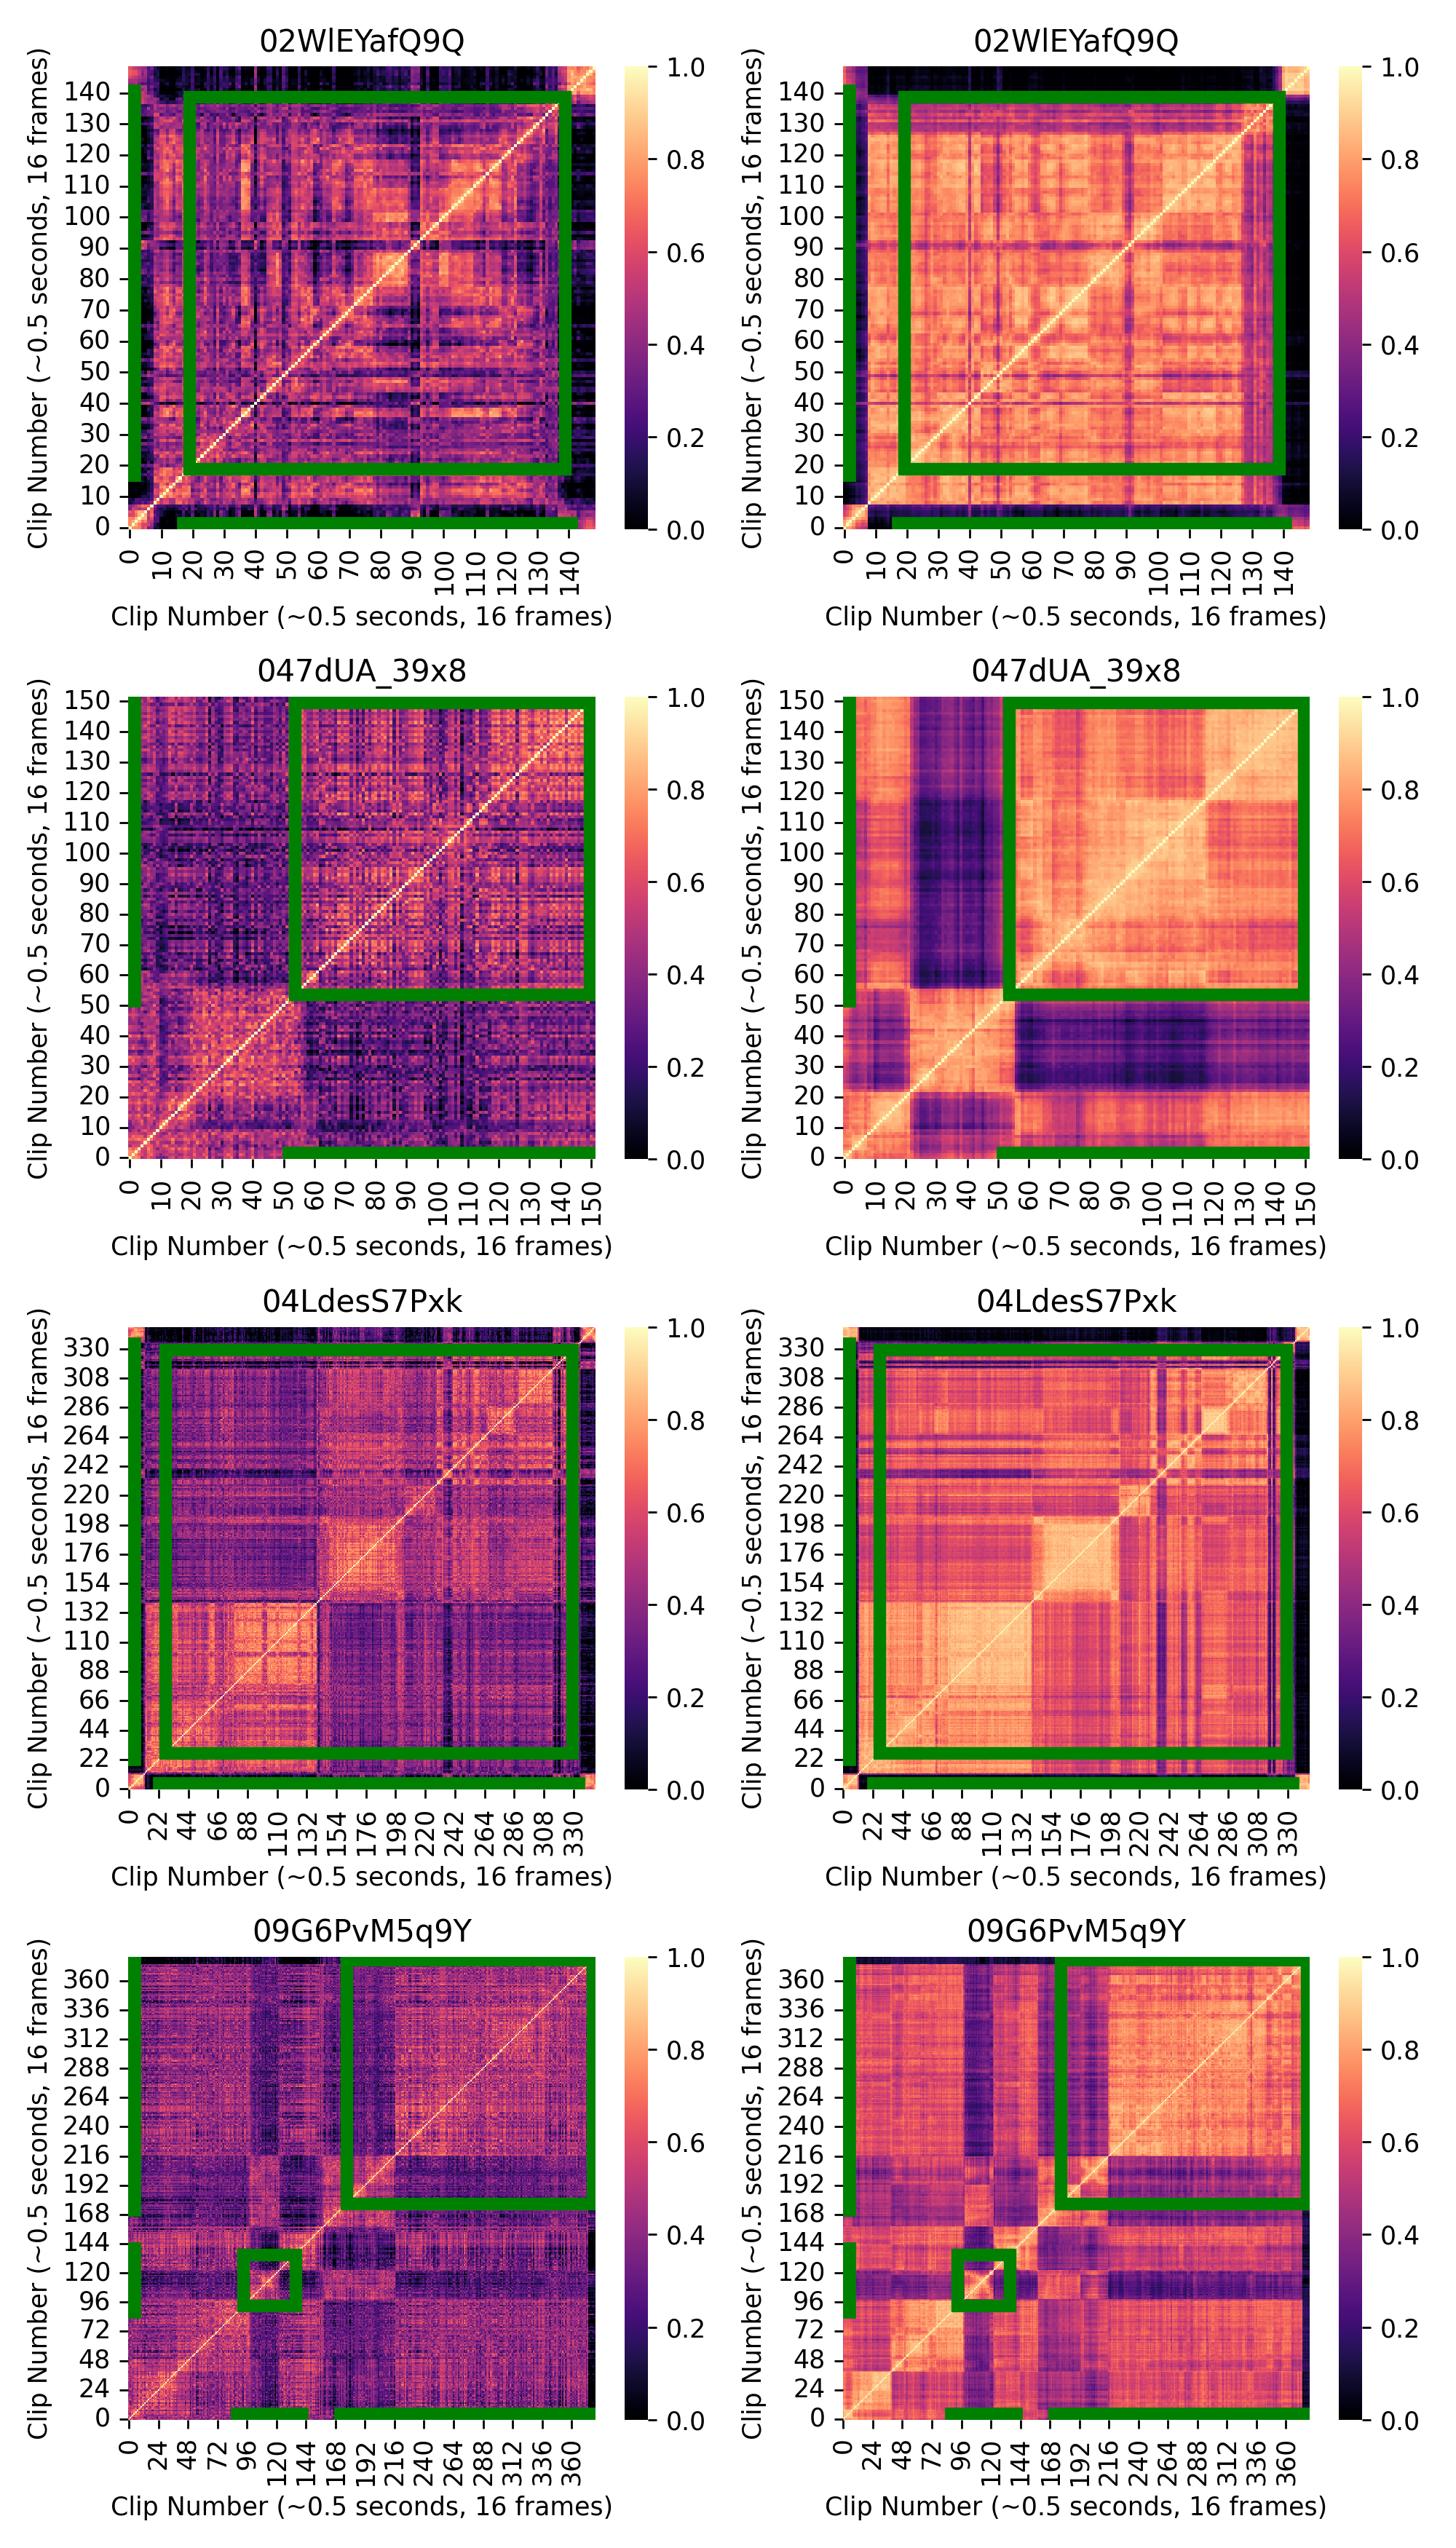
\includegraphics[width=\linewidth]{assets/img/tsp/tsp-viz-1.png}
    \end{subfigure}%
	\rulesep\rulesep
    \begin{subfigure}[b]{0.45\textwidth}
        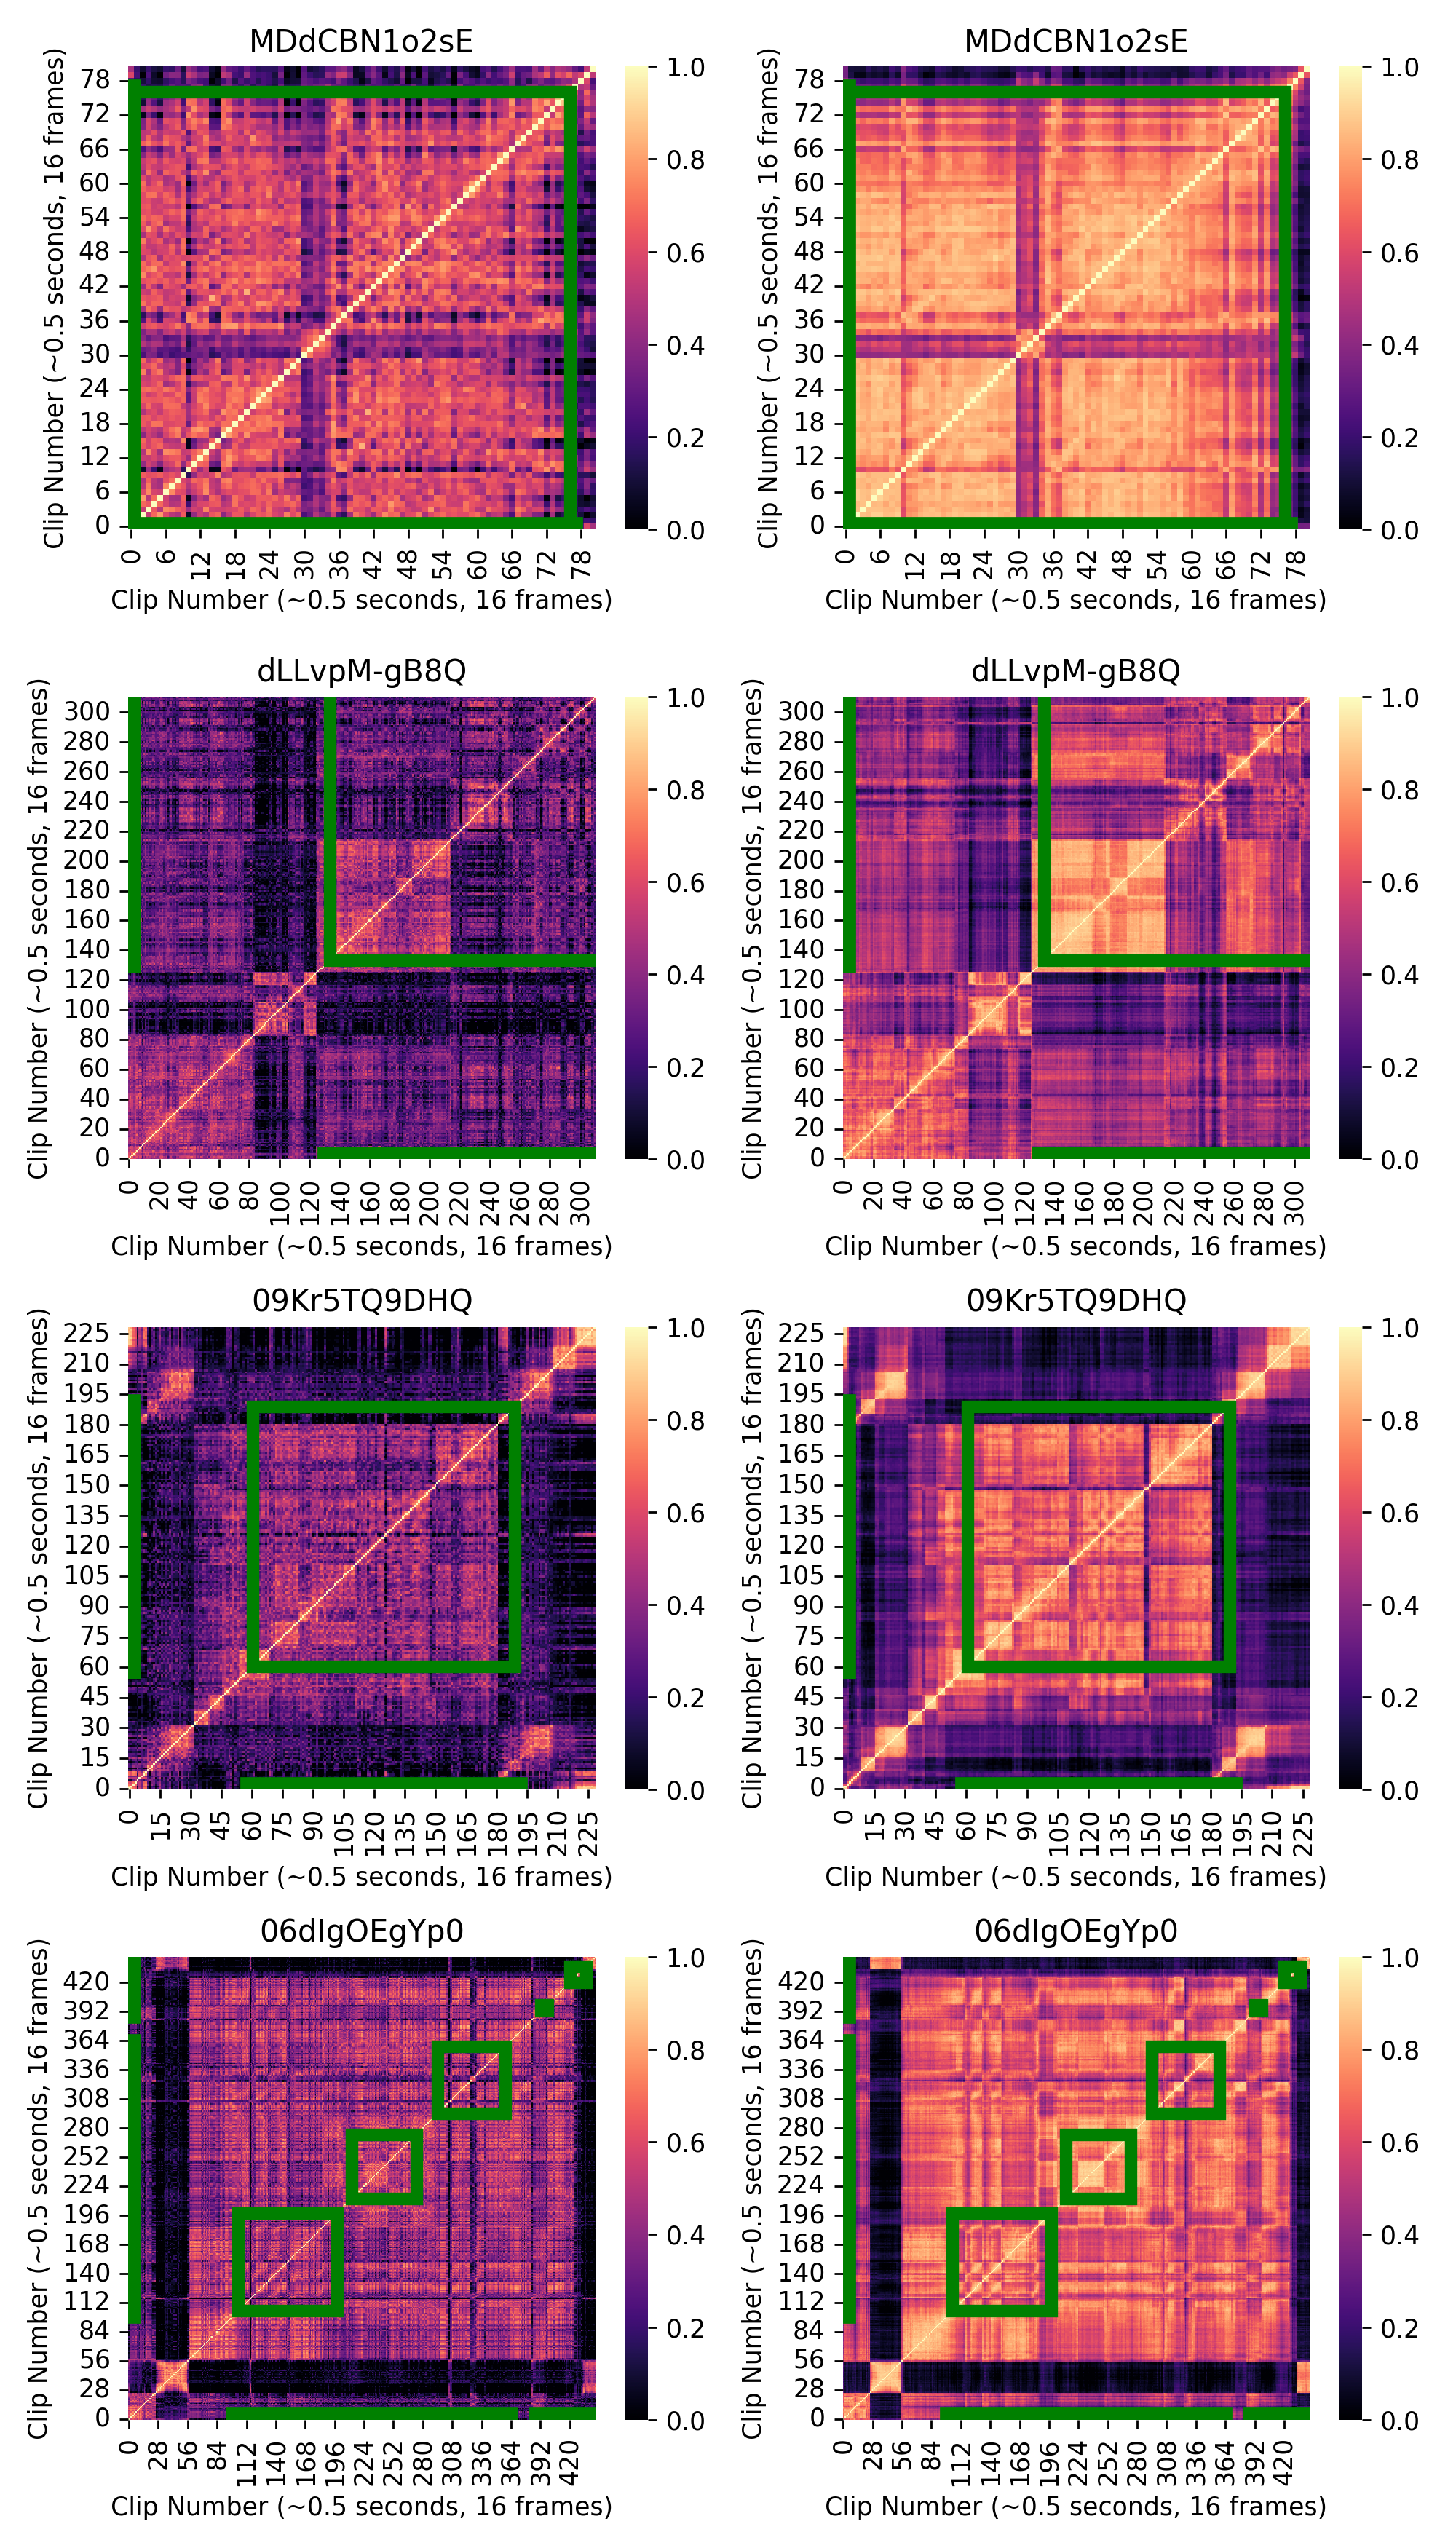
\includegraphics[width=\linewidth]{assets/img/tsp/tsp-viz-2.png}
    \end{subfigure}
    \caption{Cosine similarity matrix plots of TSP features. Each of the two columns shows features of four videos, without TSP (left) and with TSP (right). The green line segments on axes denote the ground truth segment extents, while the green square is formed by their intersection.}

	\label{fig:tsp-feats}
\end{figure}

\par We can notice that TSP features show greater similarity (closer to 1.0, with a lighter shade) within an event segment (ground truth square) than outside these squares. This indicates that the features are more representative of events. Moreover, for multiple events in a single video, we note that the intersections between distinct event segments also follow the same pattern. This is due to the following: 
\begin{itemize}
	\item TSP trains feature encoders to distinguish between action (foreground) and non-action (background) segments. Hence inter-event intersections follow a similar pattern to intra-event intersections.
	\item Most videos in the ActivityNet dataset have the same action class across multiple segments in a video, causing inter-event intersections to appear similar in the plots.
\end{itemize}

\par In order to quantitatively check the effect of TSP, we observe that the mean absolute difference between the average similarities across background regions and foreground regions increases after applying TSP. Moreover, within action regions, the variance of similarities reduces, as shown in Figure \ref{fig:tsp-action-var}.


\begin{figure}
    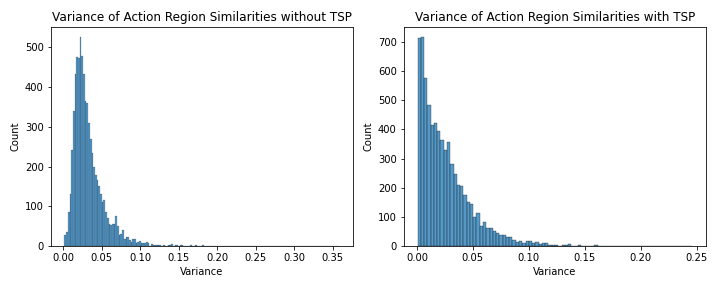
\includegraphics[width=\linewidth]{assets/img/tsp/tsp-action-sim.png}
    \caption{Histograms showing the distribution of mean similarity variance without TSP (left) and with TSP (right)}

	\label{fig:tsp-action-var}
\end{figure}

\par These observations indicate the increased temporal sensitivity of video features since action and non-action segments are more distinguished.